In questo capitolo vengono illustrate le motivazioni e i presupposti sui quali si basa il progetto e vengono presentati i principali strumenti e tecnologie utilizzati nella sua realizzazione.

\section{Ambiti di utilizzo}

%% paragraphs: cosa si intende per wireless, perché tecnologie diverse, usi in base alle funzionalità fornite, proposta di un'alternativa, perché l'alternativa è qualcosa di diverso
%% e perché può funzionare e in cosa è meglio delle esistenti
Analizzando la vasta scelta di proiettori wireless disponibili sul mercato diventa chiaro come non esista una tecnologia specifica su cui basare gli strumenti, anzi, in mancanza di uno standard non esiste neppure un accordo tra produttori su che cosa si intenda per "wireless". Proiettori di brand diversi vengono infatti pubblicizzati come dotati di funzionalità wireless che nella pratica utilizzano tecnologie molto distanti tra di loro, di fatto risultando in modalità di utilizzo variabili per l'utente.\\
Differenze in queste tecnologie riguardano molteplici fattori tra cui la tipologia di file che può essere trasmessa (documenti o video), la stabilità della connessione, il tipo di connessione richiesta, ad esempio in rete LAN privata creata ad hoc o all'interno di una rete esistente.\\
Solo alcuni modelli sono in grado di trasmettere video senza che l'utente noti rallentamenti nella riproduzione dell'immagine, la maggior parte infatti supporta solo la condivisione di documenti o immagini. \\ Quei proiettori che richiedono il setup di una rete privata per stabilire la connessione tra dispositivi, e quindi non possono collegarsi ad una rete esistente, vanno ad impegnare l'interfaccia WiFi del laptop, impedendo all'utente di avere una connessione Internet funzionante durante la proiezione, a meno che non si ricorra ad una schede di rete esterna in aggiunta per ottenere una seconda interfaccia di rete.\\
La maggior parte dei modelli inoltre necessita di hardware aggiuntivo, in particolare adattatori USB, e richiede l'installazione di applicazioni sia desktop che mobile, per funzionare.\\
Per quanto riguarda i costi, questi variano a seconda dell'approccio seguito: è possibile avere un proiettore wireless acquistandone uno che possiede il WiFi built-in oppure si può acquistare un adattatore wireless da collegare ad un tradizionale proiettore.\\
Nel primo caso un proiettore wireless-enabled può costare fino a 3000\$, mentre nel secondo caso è richiesto un costo per adattatore che va dai 50\$ ai 1300\$.\\
La soluzione proposta di seguito si presenta come alternativa alle definizioni di "proiettore wireless" date finora, con l'obiettivo di configurarsi come una soluzione di costo minore, con ampia compatibilità di sistemi operativi e in modo particolare, volta a superare le limitazioni date da quelle tipologie di prodotti che, non integrandosi in reti esistenti, impediscono all'utilizzatore la navigazione online.\\
Lo strumento proposto infatti, essendo basato esclusivamente sulla tecnologia VNC per quanto riguarda la connettività, può essere collocato tra i servizi di rete che fanno uso del semplice protocollo IP per realizzare le proprie funzionalità, utilizzando un'unica interfaccia di rete fisica.

\section{VNC}
VNC (Virtual Network Computing) è una tecnologia che consente la condivisione in remoto di desktop grafici. Può trasmettere gli eventi generati da tastiera e mouse da un ambiente grafico ad un altro, attraverso la rete, permettendo così di controllare un altro computer a distanza.\\
È basato sul protocollo di rete RFB (Remote Frame Buffer) che scambia i dati tra due computer ed è realizzato su un modello client/server: nell'utilizzo tipico un VNC client (o viewer) invia gli eventi da interpretare e un  VNC server li riceve e li trasforma in input locali; per questo motivo, i software VNC vengono spesso utilizzati per fornire assistenza remota a pc distanti nella rete.\\
\begin{figure}[ht]
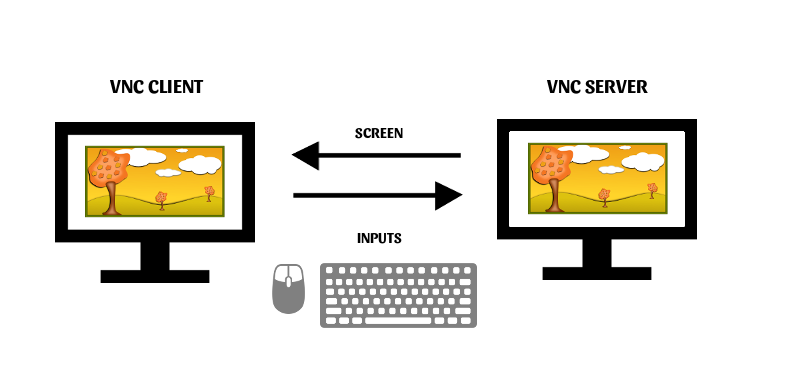
\includegraphics[width=\textwidth]{../img/vnc-client-server.png}
\centering
\caption{Interazione tra un client e un server VNC}
\end{figure}
Uno dei punti di forza di VNC è il fatto di essere indipendente dalla piattaforma, esistono implementazioni software di VNC per sistemi operativi diversi, tutte capaci di interoperare tra di loro.

\section{Raspberry Pi}

I Raspberry Pi sono una serie di mini computer single-board progettati nel Regno Unito con l'intento di diffondere nelle scuole e nei paesi in via di sviluppo le basi dell'informatica e della programmazione.
Dal 2012 ne sono state realizzate diverse versioni, nel progetto ne sono state utilizzate due, il Raspberry Pi 2 Model B e il Raspberry Pi Zero W.
    \subsection{Raspberry Pi 2}
    Fa parte della seconda generazione di Raspberry Pi, presenta una vasta dotazione di porte (USB, HDMI, Ethernet) ma manca del WiFi onboard. Nel progetto è stato dotato di WiFi attraverso un dongle USB ed utilizzato per eseguire il VNC client.
    \subsection{Raspberry Pi Zero W}
    È stato utilizzato nella seconda parte del progetto come VNC server. Manca di alcune porte rispetto al precedente, è di dimensioni molto minori ed è dotato di WiFi onboard.
\begin{figure}[ht]
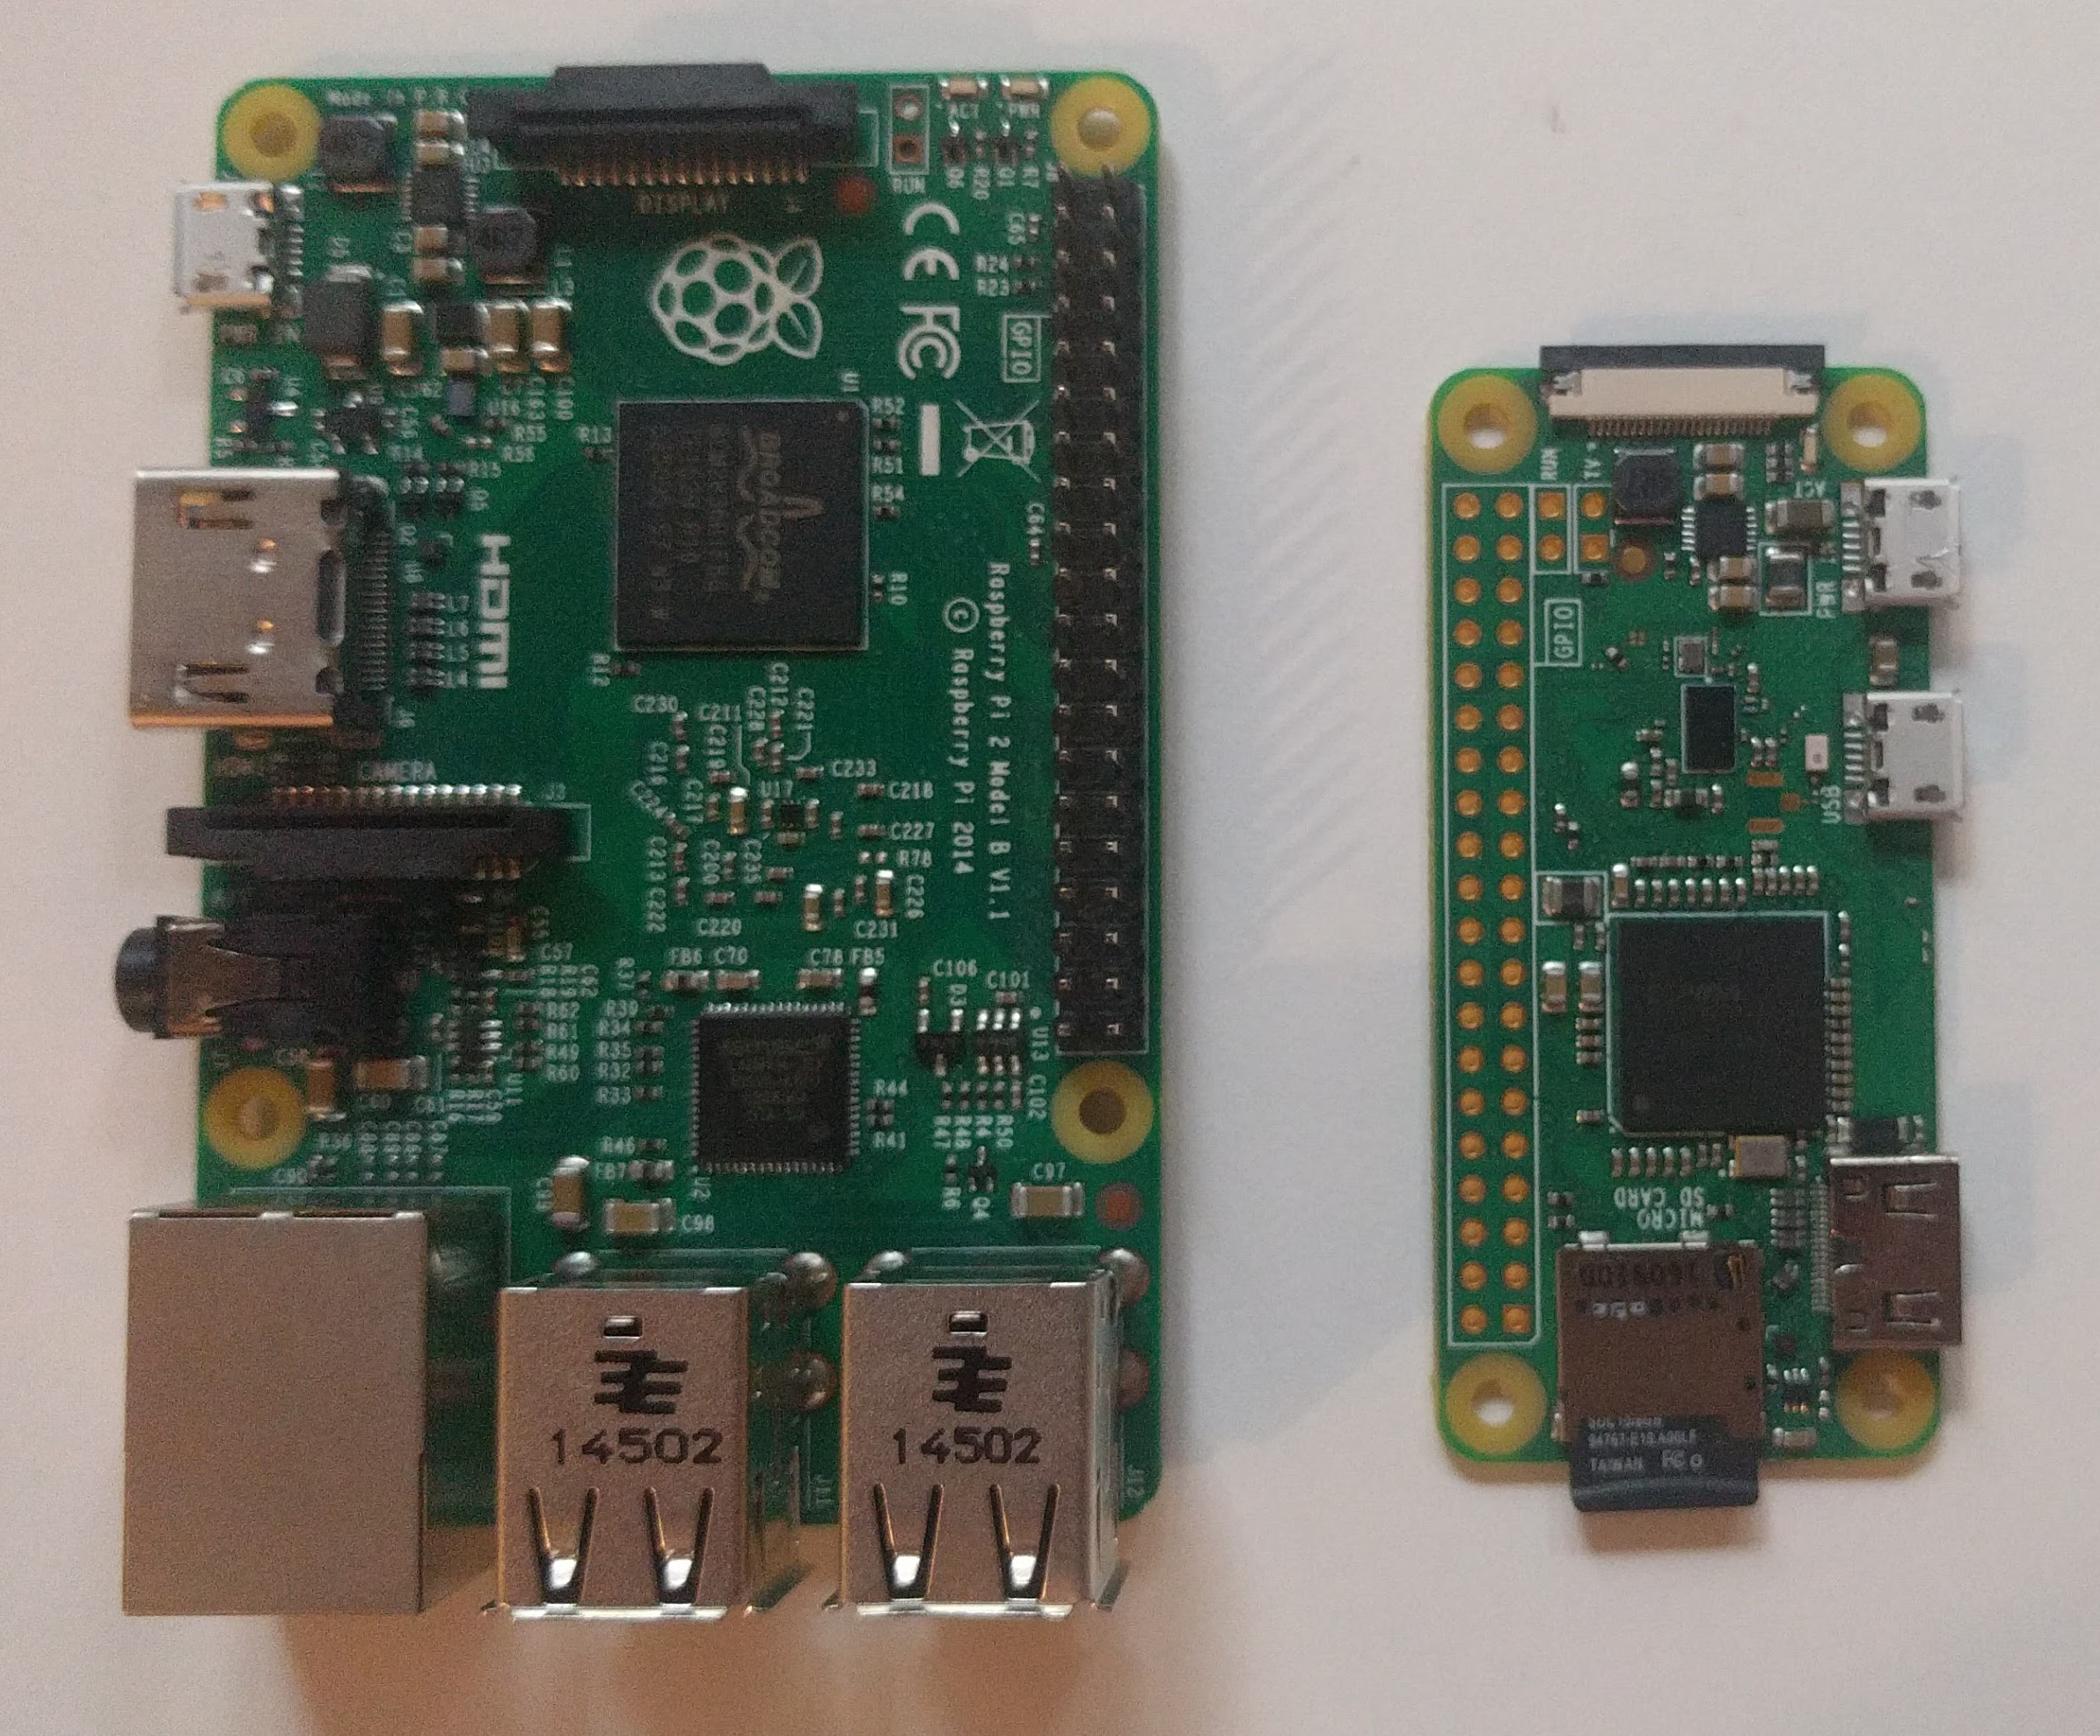
\includegraphics[width=\textwidth]{../img/pi-comparison.jpg}
\centering
\caption{Raspberry Pi 2 (a sinistra) e Zero W (a destra)}
\end{figure}
